\addcontentsline{toc}{section}{Appendix}

\chead{\textit{\nouppercase{Appendix}}}

\thispagestyle{plain} % surpress header on first page

\subsection{Appendix A} \label{appendixA}
\thispagestyle{plain} % surpress header on first page

This part explains to which extent my implementations of the NFXP and MPEC differ to the ones by \cite{Iskhakov.2016}. As already laid out in section \ref{generalsetup}, we rely entirely on open-source programs which has some implications for our methodology. The authors use matlab for the NFXP (they also implement the BHHH like this) and the modeling language AMPL in combination with the solver KNITRO for MPEC. I, on the other hand, implement everything in Python only and use IPOPT as a solver for MPEC. This alone can cause the their results and mine to differ. Additionally, for MPEC they obtain first and second order analytical derivatives of the Lagrangian as AMPL provides them using automatic differentiation. While there are tools such as JAX\footnote{See https://github.com/google/jax .} that provide analytical derivatives via automatic differentiation for code written in Python, these restrict the code to have a certain form which would have involved rewriting main parts of the existing code. This might be an interesting extension of the package for later but is out of bounds for this thesis. I decided therefore to at least code up the first order derivative by hand and pass it on to IPOPT. The fact that the Hessian has to be approximated can potentially influence the results strongly. \citeauthor{Iskhakov.2016} also give sparsity patterns of the two derivatives to KNITRO in order to conserve memory and increase speed. This is not done in my implementation. Another practical difference comes from the fact that KNITRO and IPOPT rely on different stopping criteria which makes it impossible to exactly replicate the setup for KNITRO with IPOPT. For the NFXP there are also some differences. My BHHH as well as the switching from contraction to N-K iterations has other tolerances. On top of that, \citeauthor{Iskhakov.2016} allow the fixed point algorithm to switch back from N-K to contraction steps when a certain criteria is met. This flexibility is not implemented in my code.

In the light of that, the algorithms by \citeauthor{Iskhakov.2016} are slightly more complex and robust which seems to affect the number of iterations and function evaluations for MPEC and especially the amount of contraction and N-K steps needed in the case of the NFXP. This can be observed in Table \ref{table1}. Although one should mention that the more comparable implementation of MPEC in which \cite{Su.Judd.2012} use matlab as the modeling language and KNITRO with only first order analytical derivatives as solver seems to be inferior to my implementation when looking at the number of iterations and function evaluations needed \footnote{To see this, have a look at Table II on page 2228 of \cite{Su.Judd.2012}. One has to be cautious, though, as their implementation differs from mine in the sense that they do not recenter the expected value function.}. For an additional sanity check I provide the mean and standard deviations of the estimated cost parameters across the Monte Carlo simulations outlined in section \ref{generalsetup}. These are meaningful as \cite{Su.Judd.2012} argue that this simulation actually constitutes a parametric bootstrap procedure. The two statistics are provided for both my implementations and additionally for the NFXP of \citeauthor{Iskhakov.2016}. These results were not published but had to be obtained by me using their matlab replication code. Unfortunately, their code does not run through but only did with some additional changes. This should make one a bit cautious regarding these results. All of those results are presented in the table below in which can be seen that apart from when $\beta$ equals $0.995$ the results of all three approaches are very similar. \paragraph{}

\begin{table}[H]
	\centering
	\caption{Comparison to the Results of Iskhakov et al. (2016)}
	\begin{tabular}{l c c c c}
		\toprule\midrule
		& & & RC & $\theta_{11}$ \\
		\cmidrule{4-5}
		$\beta$ & Implementation & True Values: & $\mathbf{11.726}$ & $\mathbf{2.457}$ \\ \midrule
		0.975 & MPEC & Mean & 11.908 & 2.507 \\
		& & Std. Dev. & (1.517) & (0.486) \\
		& NFXP & Mean & 11.908 & 2.507 \\
		& & Std. Dev. & (1.517) & (0.468) \\
		& NFXP Iskhakov & Mean & 11.914 & 2.508 \\
		& & Std. Dev. & (1.517) & (0.468) \\ \midrule
		0.985 & MPEC & Mean & 11.986 & 2.534 \\
		& & Std. Dev. & (1.457) & (0.452) \\
		& NFXP & Mean & 11.986 & 2.534 \\
		& & Std. Dev. & (1.457) & (0.452) \\
		& NFXP Iskhakov & Mean & 11.991 & 2.535 \\
		& & Std. Dev. & (1.457) & (0.452) \\ \midrule
		0.995 & MPEC & Mean & 11.891 & 2.508 \\
		& & Std. Dev. & (1.384) & (0.440) \\
		& NFXP & Mean & 11.891 & 2.508 \\
		& & Std. Dev. & (1.384) & (0.440) \\
		& NFXP Iskhakov & Mean & 11.191	& 2.902 \\
		& & Std. Dev. & (1.188) & (0.473) \\ \midrule
		0.999 & MPEC & Mean & 11.874 & 2.513 \\
		& & Std. Dev. & (1.347) & (0.444) \\
		& NFXP & Mean & 11.874 & 2.513 \\
		& & Std. Dev. & (1.347) & (0.444) \\
		& NFXP Iskhakov & Mean & 11.876	& 2.513 \\
		& & Std. Dev. & (1.346) & (0.444) \\ \midrule
		0.9995 & MPEC & Mean & 11.849 & 2.509 \\
		& & Std. Dev. & (1.343) & (0.445) \\
		& NFXP & Mean & 11.847 & 2.508 \\
		& & Std. Dev. & (1.343) & (0.445) \\
		& NFXP Iskhakov & Mean & 11.849 & 2.509 \\
		& & Std. Dev. & (1.342) & (0.445) \\ \midrule
		0.9999 & MPEC & Mean & 11.815 & 2.498 \\
		& & Std. Dev. & (1.319) & (0.431) \\
		& NFXP & Mean & 11.815 & 2.499 \\
		& & Std. Dev. & (1.319) & (0.431) \\
		& NFXP Iskhakov & Mean & 11.817	& 2.499 \\
		& & Std. Dev. & (1.319) & (0.431) \\ \bottomrule
	\end{tabular}
\end{table}

My implementations overestimate the true parameter slightly for $RC$ while coming gradually closer to the true value with increasing $\beta$. This pattern can also be seen in Table I of \cite{Su.Judd.2012} (who base their analysis on the same data generating process) which makes me confident that my results are correct. It seems like for $\beta = 0.995$ the NFXP Iskhakov is trapped in another local minimum that causes it to overestimate the true $\theta_{11}$ by a lot and suddenly underestimate the true $RC$. As mentioned before, this is likely to be caused by the fact that their code did not run through and it is not obviously clear whether the setup in the code is exactly like the one the published results are based on.

\subsection{Appendix B: Tables}

\begin{table}[H]
	\centering
	\caption{Correlation between Parameter Estimates}
	\label{correlation}
	\begin{tabular}{l | c c c c c c c}
		\toprule\midrule
		& $\hat{RC}$ & $\hat\theta_{11}$ & $\hat\theta_{30}$ & $\hat\theta_{31}$ & $\hat\theta_{32}$ & $\hat\theta_{33}$ \\ \midrule
		$\hat{RC}$ & 1.0 & 0.97 & -0.04 & -0.01 & 0.00 & 0.15 \\
		$\hat\theta_{11}$ & 0.97 & 1.0 & -0.02 & -0.03 & 0.01 &	0.14 \\
		$\hat\theta_{30}$ &	-0.04 &	-0.02 &	1.0	& -0.26 & -0.31 & -0.07 \\
		$\hat\theta_{31}$ &	-0.01 &	-0.03 &	-0.26 &	1.0 & -0.82 & -0.06 \\
		$\hat\theta_{32}$ &	0.00 & 0.01 & -0.31 & -0.82 & 1.0 &	-0.12 \\
		$\hat\theta_{33}$ &	0.15 & 0.14 & -0.07 & -0.06 & -0.12 & 1.0 \\
		\bottomrule
	\end{tabular}
\end{table}


\begin{table}[H]
	\centering
	\caption{The Specifications for the Sensitivity Simulation}
	\label{table4}
	\begin{tabular}{l c c c c}
		\toprule\midrule
		Specification & $\beta$ & Cost Function & Grid Size & Analytical \\
		& & & & Gradient \\ \midrule
		0 & 0.975 & linear& 100& Yes\\
		1&0.975& linear& 100& No\\
		2&0.975& linear& 200& Yes\\
		3&0.975& linear& 200& No\\
		4&0.975& linear& 400& Yes\\
		5&0.975& linear& 400& No\\
		6&0.975& quadratic& 100& Yes\\
		7&0.975& quadratic& 100& No\\
		8&0.975& quadratic& 200& Yes\\
		9&0.975& quadratic& 200& No\\
		10&0.975& quadratic& 400& Yes\\
		11&0.975& quadratic& 400& No\\
		12&0.975& cubic& 100& Yes\\
		13&0.975& cubic& 100& No\\
		14&0.975& cubic& 200& Yes\\
		15&0.975& cubic& 200& No\\
		16&0.975& cubic& 400& Yes\\
		17&0.975& cubic& 400& No\\
		18&0.985& linear& 100& Yes\\
		19&0.985& linear& 100& No\\
		20&0.985& linear& 200& Yes\\
		21&0.985& linear& 200& No\\
		22&0.985& linear& 400& Yes\\
		23&0.985& linear& 400& No\\
		24&0.985& quadratic& 100& Yes\\
		25&0.985& quadratic& 100& No\\
		26&0.985& quadratic& 200& Yes\\
		27&0.985& quadratic& 200& No\\
		28&0.985& quadratic& 400& Yes\\
		29&0.985& quadratic& 400& No\\
		30&0.985& cubic& 100& Yes\\
		31&0.985& cubic& 100& No\\
		32&0.985& cubic& 200& Yes\\
		33&0.985& cubic& 200& No\\
		34&0.985& cubic& 400& Yes\\
		35&0.985& cubic& 400& No\\
		\bottomrule
	\end{tabular}
\end{table}


\subsection{Appendix B: Figures}

\begin{figure}[H]
	\caption{The QoI when varying the Cost Function (BHHH)}
	\vspace*{-4mm}
	\centering
	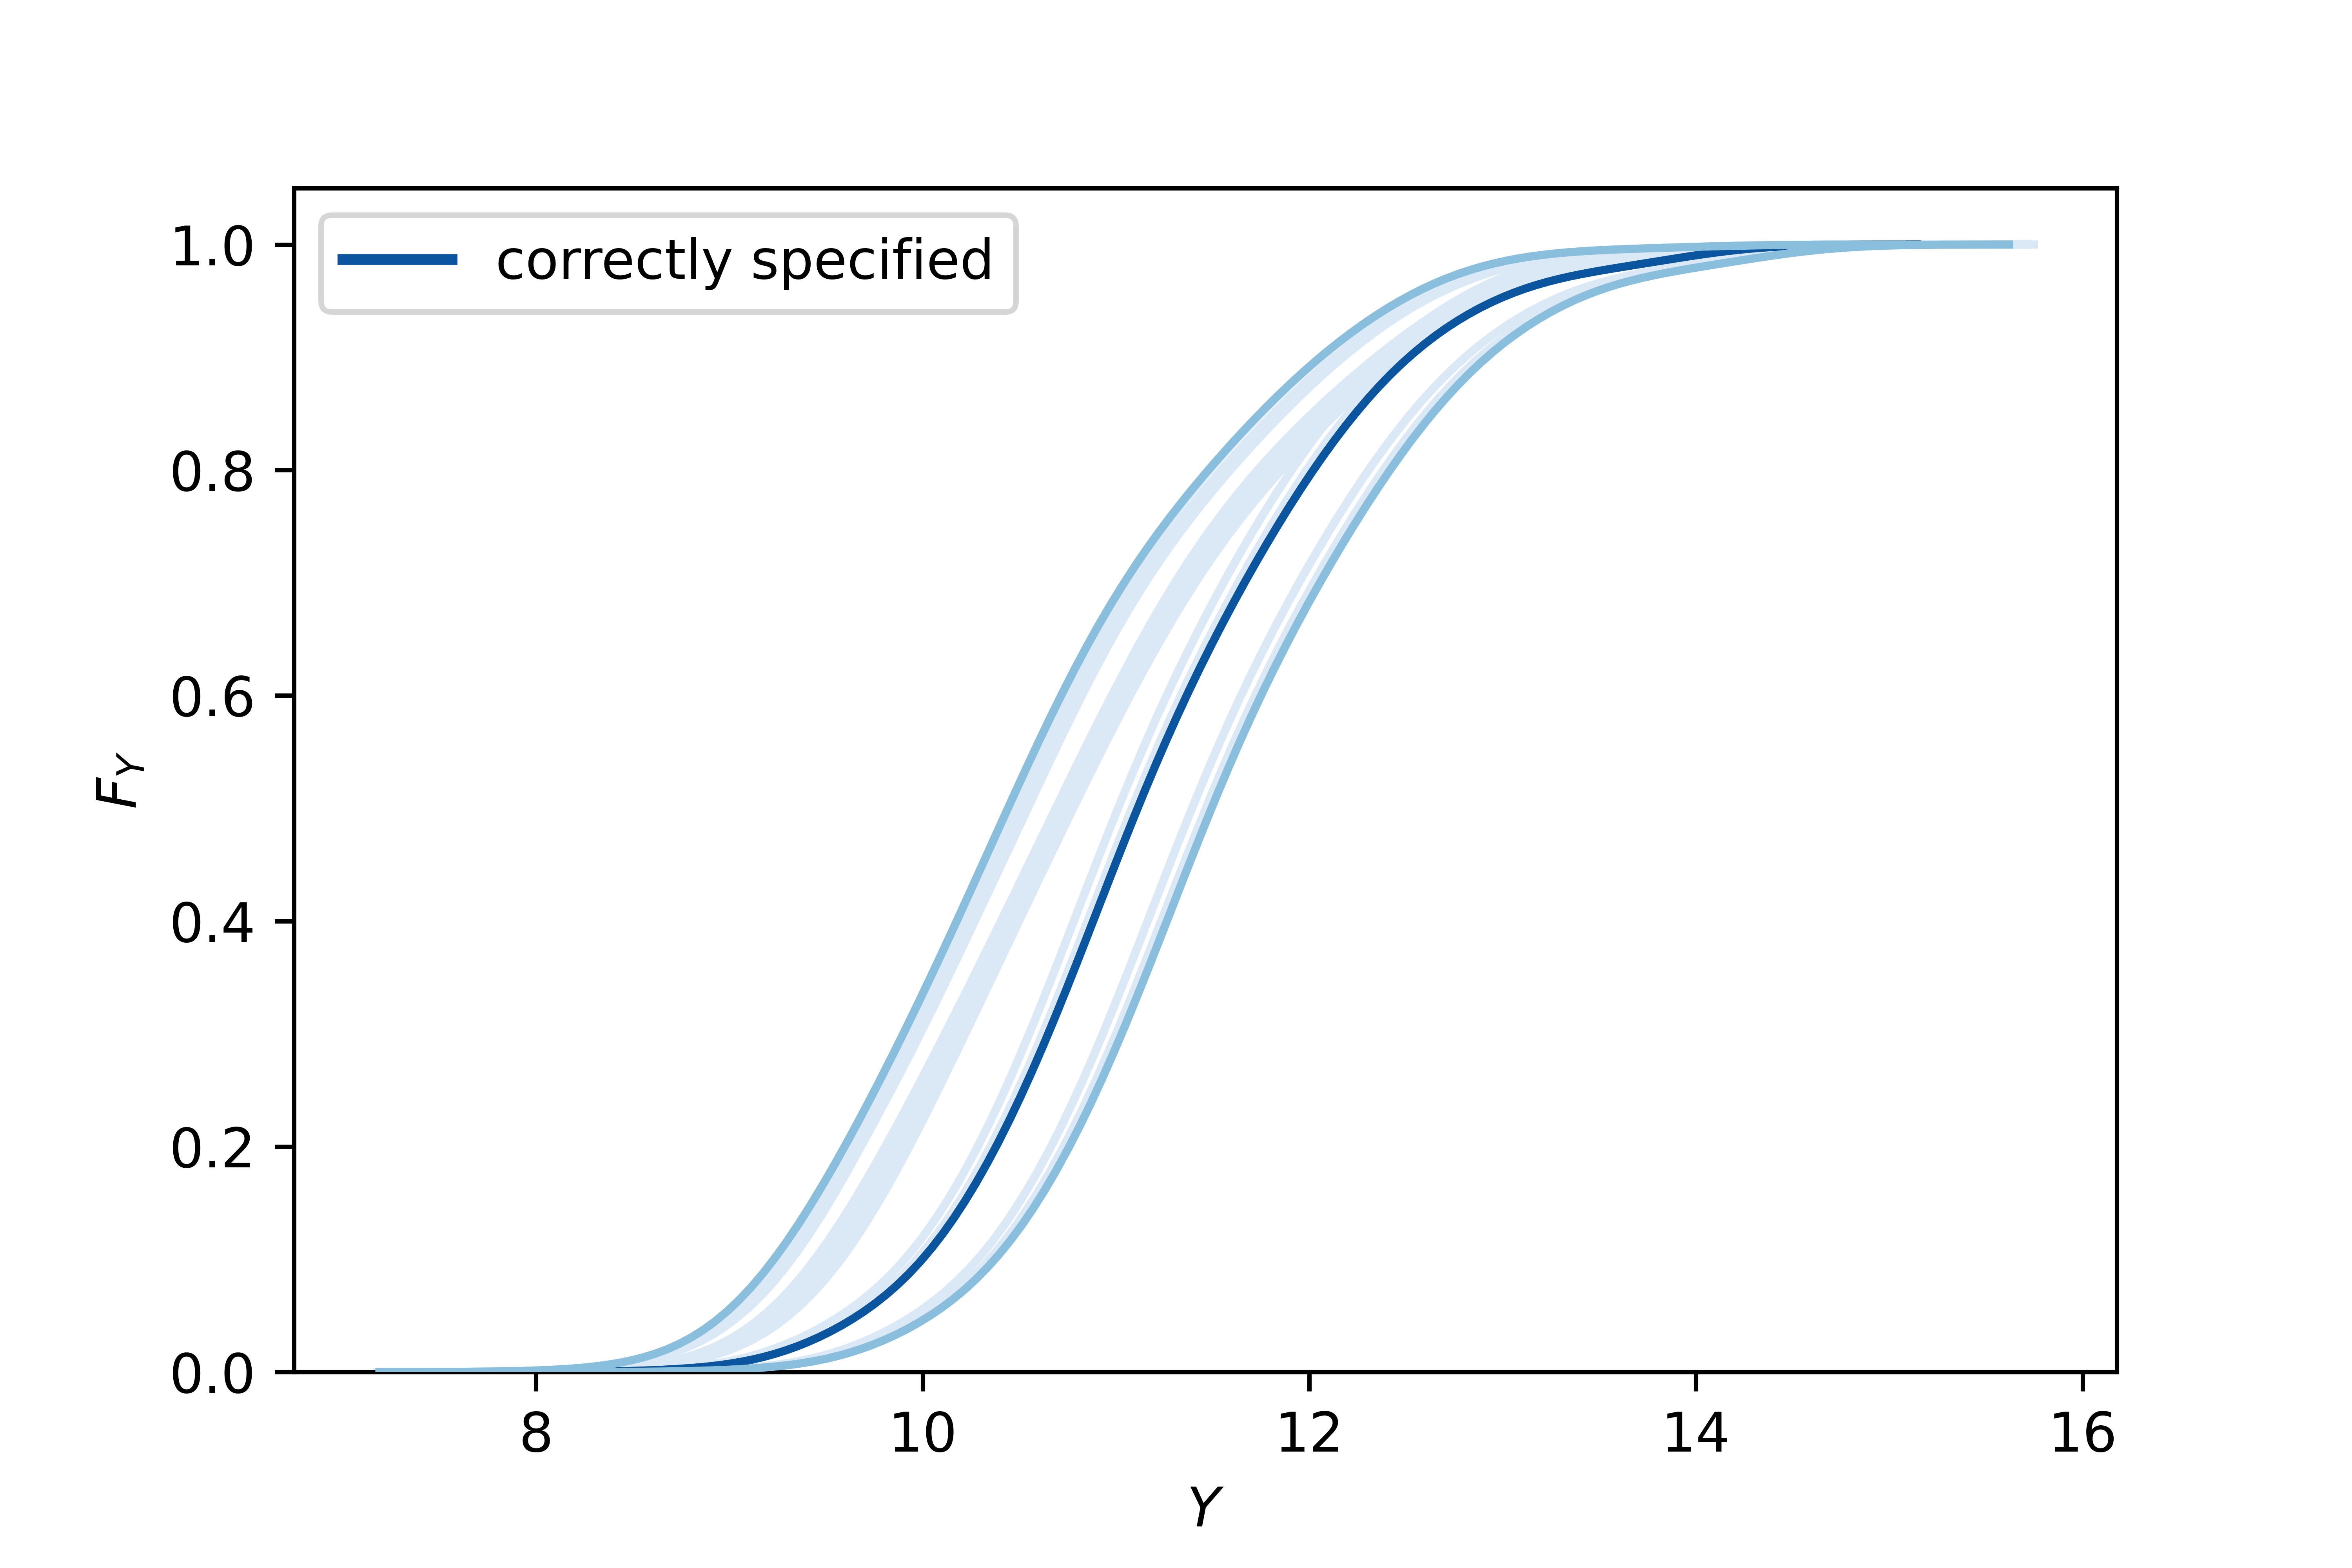
\includegraphics[scale=0.9]{../figures/figure_12.png}
	\label{figure12}
\end{figure}

\begin{figure}[H]
	\caption{The PDF and CDF of the QoI with the NFXP}
	\vspace*{-4mm}
	\centering
	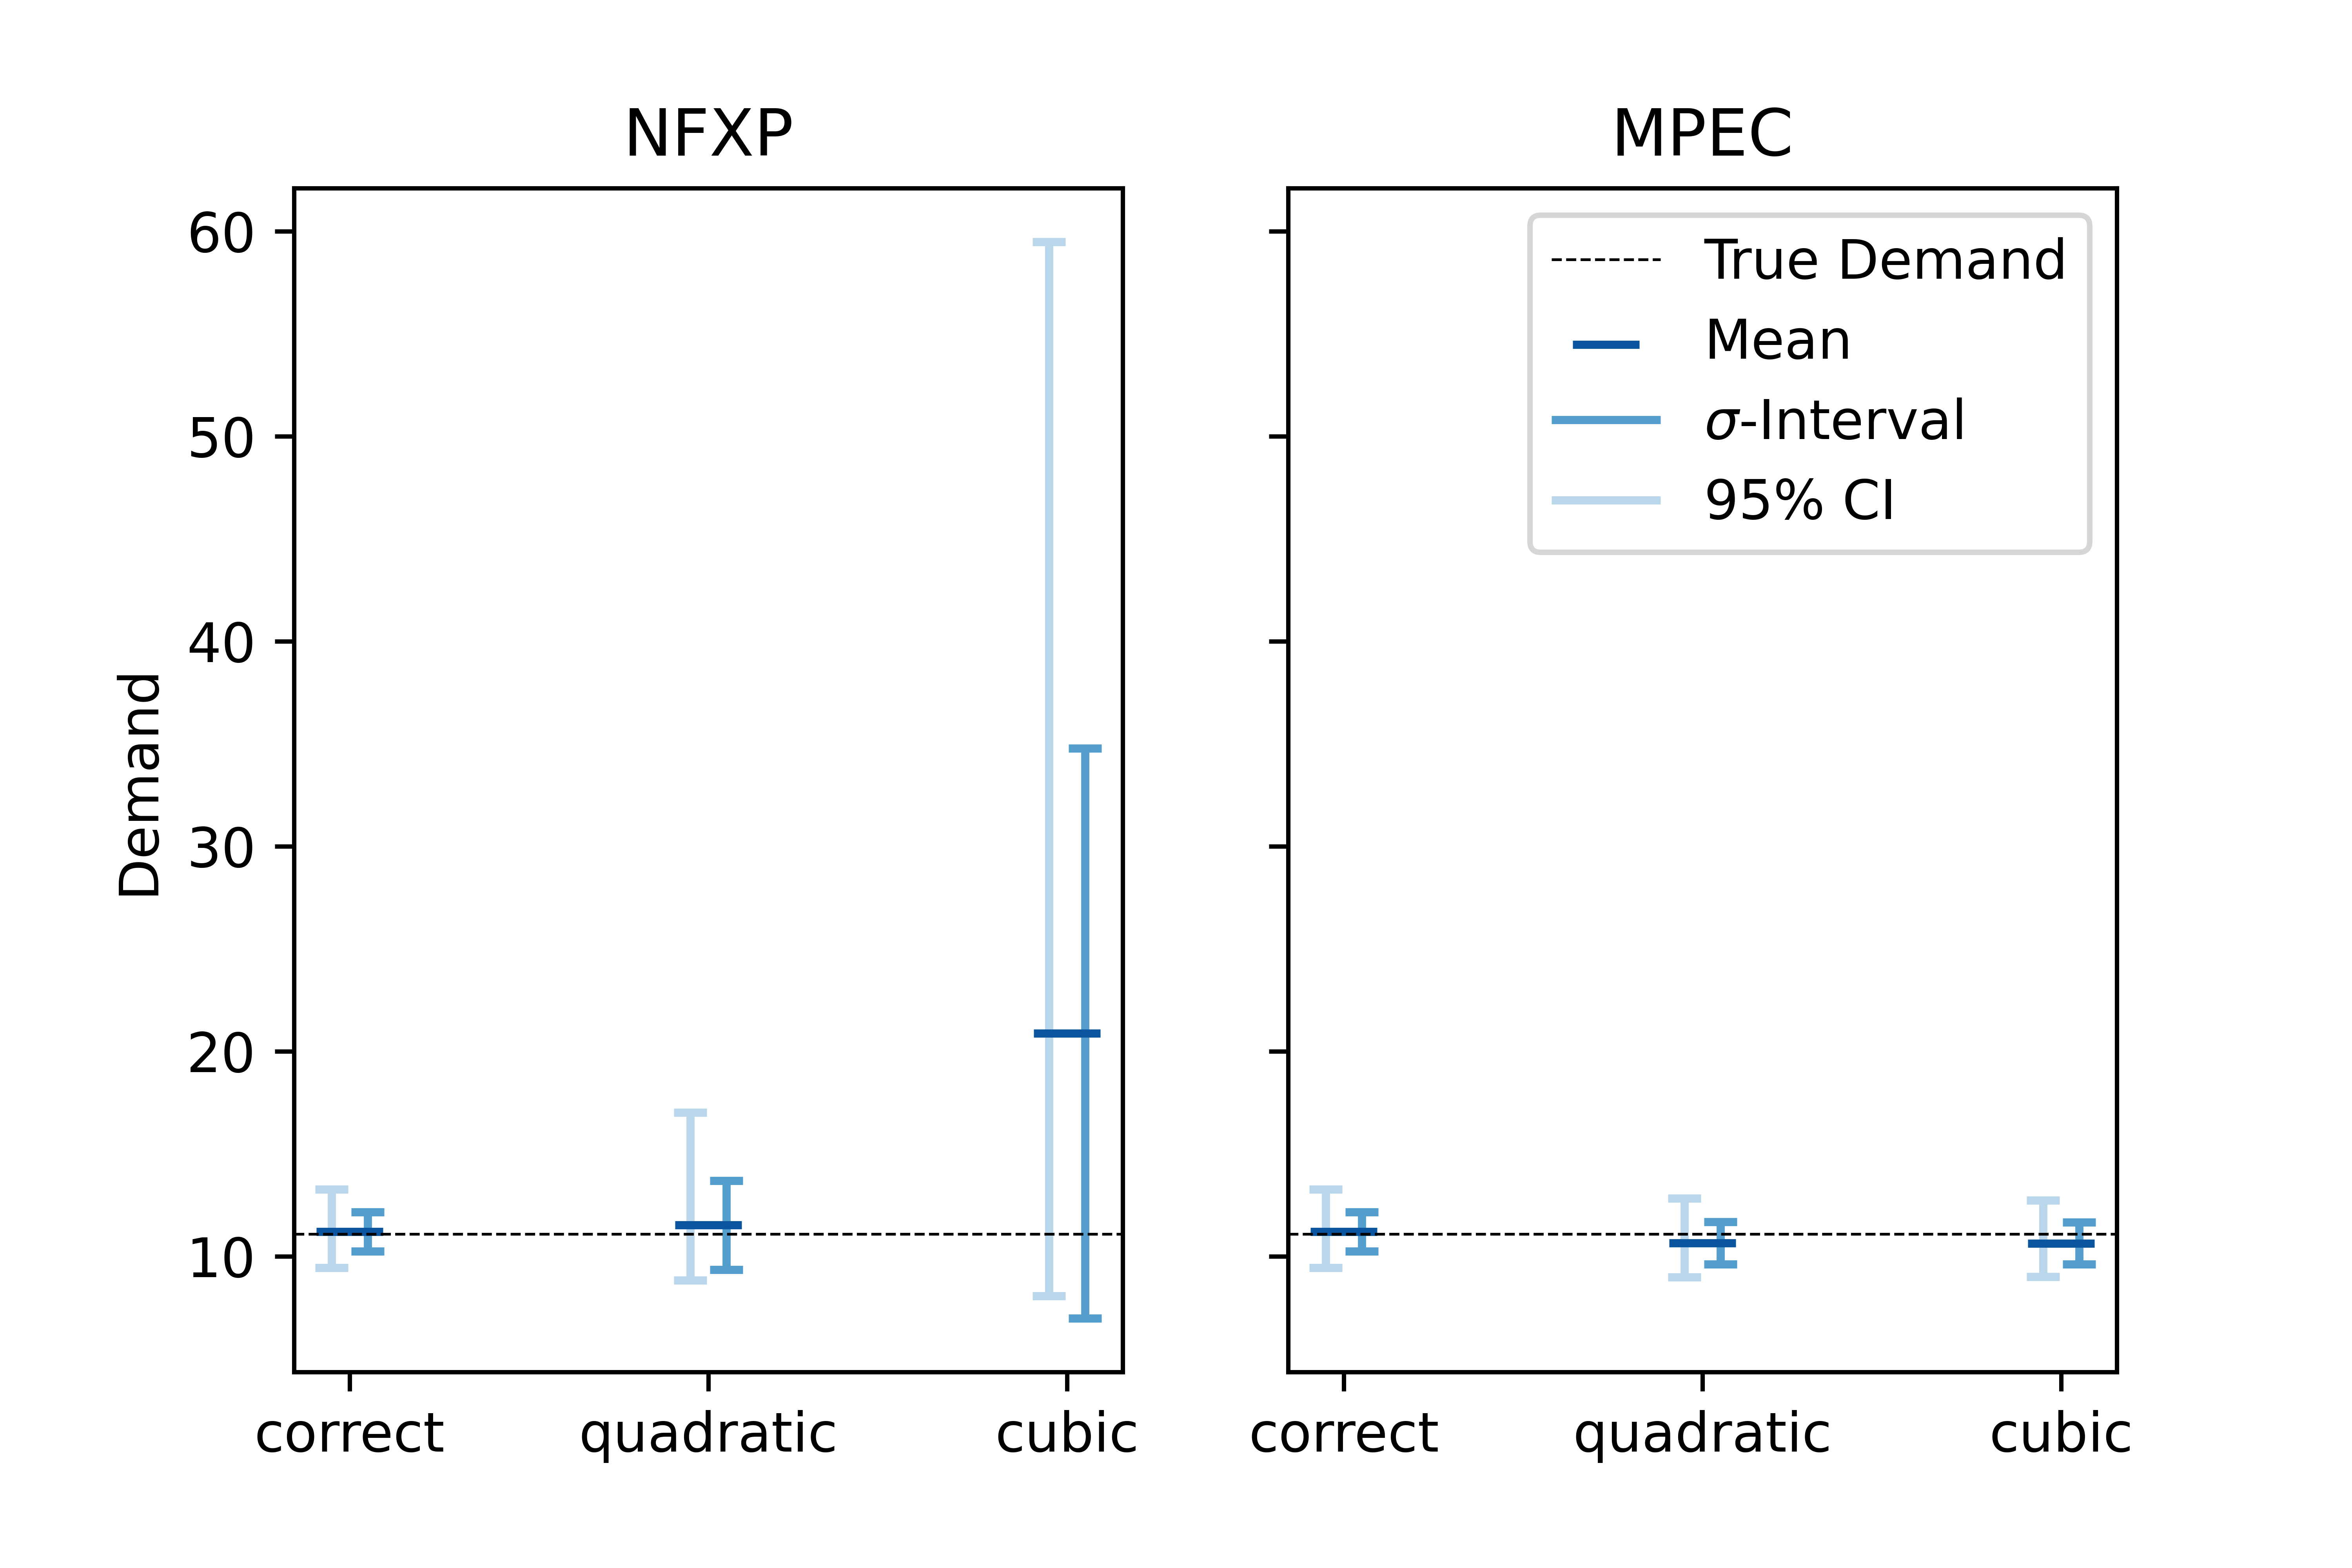
\includegraphics[scale=0.9]{../figures/figure_13.png}
	\label{figure13}
\end{figure}
